\section{Feature Engineering}\label{sec:fe}

We hand the modelling phase \nFeatures features (Table~\ref{tab:feature-list}), every one decided on training rows only, none of which can leak the answer, and none of which is an exact or near-exact linear combination of the others. The final tables are \file{nhis_lung_cancer_model_ready.csv} (original units) and \file{nhis_lung_cancer_model_ready_scaled.csv} (standardised), and every keep/drop decision, with its reason, is recorded in \file{final_features.csv}, so anyone can audit it.

\subsection{Features we created}\label{sec:created}

\begin{table}[htbp]
\centering\small
\caption{Engineered and joined features, with their definition and rationale.}\label{tab:engineered}
\begin{tabularx}{\textwidth}{@{}>{\raggedright\arraybackslash}p{3.9cm} >{\raggedright\arraybackslash}p{3.7cm} >{\raggedright\arraybackslash}X@{}}
\toprule
Feature & Definition & Why we built it \\
\midrule
\texttt{screening\_age\_smoker} & 1 if aged 50--80 and ever smoked & a proxy for the official USPSTF screening group; Fig.~\ref{fig:agesmoking} shows that risk piles up exactly there. Without pack-years it is only an approximation (an interaction feature built from domain knowledge) \\
\texttt{comorbidity\_count} & number of the 5 conditions (0--5) & one number for overall health burden, used in the EDA (Tables~\ref{tab:prof-conditions}--\ref{tab:cases}, Fig.~\ref{fig:numeric}, Fig.~\ref{fig:corr}); not a model feature, because it is the exact sum of the five condition flags (dropped by rule 4, \S\ref{sec:selection}) \\
\texttt{ever\_smoker} & current or former smoker & simple exposure flag, used for the odds ratio in RQ1 (dropped from the model set as redundant, \S\ref{sec:selection}) \\
\texttt{age\_group} & 18--44, 45--54, 55--64, 65--74, 75+ & used for reporting, the age $\times$ smoking table and the age-adjusted tests; exact age is kept for the model instead \\
\texttt{pm25\_mean}, \texttt{smoking\_rate}, \texttt{lung\_cancer\_incidence} & regional values joined on region + year (\S\ref{sec:integration}) & environmental and baseline-risk context for RQ3 \\
\bottomrule
\end{tabularx}
\end{table}

\subsection{Encoding and imputation}\label{sec:encoding}

\begin{itemize}
  \item \textbf{One-hot encoding} for the nominal variables (sex, race/ethnicity, region, smoking status) and for the grouped ordinal ones (education, income, general health, BMI, age group). We chose one-hot over label encoding so the model never assumes a false order or false equal spacing between categories (for example that ``Asian'' is ``greater'' than ``Black''). A complete set of dummies always adds up to 1, which makes a linear model impossible to fit, so the model-ready file drops one \textbf{reference category} per group and every other dummy is read relative to it: race/ethnicity \emph{White} (the largest group), education \emph{High school / GED}, income \emph{High} (four times the poverty line or more), BMI \emph{Healthy}, general health \emph{Excellent}, smoking status \emph{Never}; for sex (\emph{Male}) and region (\emph{West}) the reference was already dropped by the near-duplicate rule. The choice is recorded for every dummy in \file{final_features.csv}.
  \item \textbf{Unknown answers and the reference group.} \emph{Unknown} categories that survive selection (education, BMI) are kept as their own dummy. For smoking status, the small \emph{Unknown} dummy was dropped as a near-duplicate of \file{screening_age_smoker_unknown} ($r = 0.96$), so the 2.6\% of adults with an unknown smoking status now fall into the \emph{Never} reference group and are identified only by \file{screening_age_smoker_unknown}, which is therefore kept (\S\ref{sec:final}). The same happens to the 0.04\% with unknown general health (reference \emph{Excellent}).
  \item \textbf{Missing values} become an explicit Unknown category instead of being dropped or guessed.
  \item \textbf{Binary health columns} stay 0/1, with missing values set to 0 plus an \file{_unknown} flag; the flags for very rare gaps are later removed by the near-constant filter (\S\ref{sec:selection}).
  \item \textbf{Age} is filled with the training median (54 years); the \file{age_missing} flag created at the same time (0.24\% of adults) is later removed by the near-constant filter (\S\ref{sec:selection}).
\end{itemize}

\subsection{Scaling}\label{sec:scaling}

Four numeric features use completely different units: age in years, PM2.5 in \textmu g/m$^3$, smoking prevalence in \%, and incidence per 100,000. (The 0--5 comorbidity count is no longer a model feature, \S\ref{sec:selection}.) Distance-based and regularised models are sensitive to these scales, so we standardise them with a \file{StandardScaler} fitted on training rows only. Binary columns are already on a 0--1 scale, so we leave them alone and keep them interpretable.

\begin{table}[htbp]
\centering\small
\caption{Scaler parameters learned on the \nTrain training rows, and the mean of each scaled column on the test rows.}\label{tab:scaler}
\begin{tabular}{lrrr}
\toprule
Column & \makecell[b]{Training\\{}mean} & \makecell[b]{Training\\{}SD} & \makecell[b]{Scaled\\{}test mean} \\
\midrule
age & 52.81 & 18.33 & $-$0.002 \\
pm25\_mean & 7.289 & 0.763 & 0.006 \\
smoking\_rate & 14.475 & 2.078 & $-$0.001 \\
lung\_cancer\_incidence & 67.31 & 12.50 & 0.019 \\
\bottomrule
\end{tabular}

\end{table}

\subsection{Feature selection}\label{sec:selection}

We went from \nCandidates candidates to \nFeatures features, applying the filter pass from the course~\cite{larose,louati} on training rows only, in this order (Table~\ref{tab:selection}):

\begin{table}[htbp]
\centering\small
\caption{Feature-selection rules and the features each rule removed (\nDropped in total). Never candidates: \texttt{person\_id} (identifier), \texttt{split} (train/test label), \texttt{survey\_weight} (a sampling weight, not a property of the person) and \texttt{CANEV\_A} (reveals the answer). \texttt{sex\_Male} and \texttt{region\_West}, dropped by rule 3, also serve as the reference categories of sex and region.}\label{tab:selection}
\begin{tabularx}{\textwidth}{>{\raggedright\arraybackslash}p{5.2cm} r >{\raggedright\arraybackslash}X}
\toprule
Rule & Dropped & Features \\
\midrule
1. Redundant by construction & 8 & ever\_smoker, ever\_smoker\_unknown, age\_group\_18-44, age\_group\_45-54, age\_group\_55-64, age\_group\_65-74, age\_group\_75+, age\_group\_Unknown \\
2. Constant in training rows & 0 & -- \\
2b. Near-constant: more than 99.5\% of training rows share one value & 8 & age\_missing, copd\_unknown, asthma\_unknown, hypertension\_unknown, heart\_disease\_unknown, diabetes\_unknown, sex\_Unknown, general\_health\_Unknown \\
3. Near-duplicates: $|r| > 0.95$ with a column already kept & 3 & sex\_Male, region\_West, smoking\_status\_Unknown \\
4a. Exact linear combination of other features (VIF = $\infty$) & 1 & comorbidity\_count \\
4b. Reference category of each one-hot group & 6 & race\_ethnicity\_White, education\_High school / GED, income\_group\_High, general\_health\_Excellent, bmi\_category\_Healthy, smoking\_status\_Never \\
4c. Near-collinear block (region dummies vs regional columns) & 3 & region\_Midwest, region\_Northeast, region\_South \\
\midrule
Total dropped & 29 & 38 features kept \\
\bottomrule
\end{tabularx}

\end{table}

The near-constant rule removes columns that describe fewer than 1 adult in 200 (for example, ``COPD answer unknown'' applies to 0.06\% of adults). Such columns add almost no information but add dimensions -- the curse of dimensionality discussed in the course. We deliberately did not use target-based filtering to drop weak features: with a \sampleRate\% outcome, univariate relevance is unstable, and interactions (such as age $\times$ smoking) can make individually weak features useful. Relevance is instead checked in \S\ref{sec:mi} and will be tested by ablation in the modelling phase.

\textbf{Rule 4: dependencies spread over several columns (VIF).} Rules 1--3 compare columns one pair at a time, so they cannot see a column that is a combination of \emph{several} others. The variance inflation factor can: $\mathrm{VIF}_j = 1 / (1 - R^2_j)$, where $R^2_j$ comes from regressing feature $j$ on all the other features (with an intercept) on the training rows. $\mathrm{VIF} = 1$ means feature $j$ is unrelated to the others, $\mathrm{VIF} > 10$ is the usual alarm level, and $\mathrm{VIF} = \infty$ means an exact linear dependency. After rules 1--3, \nInfVIF of the \nFeaturesBefore features had an infinite VIF and \nVIFaboveTenBefore a VIF above 10 (Table~\ref{tab:vif}; \file{results/tables/vif_before.csv}). The causes were the comorbidity count (the sum of five flags) and the four complete one-hot groups (race, education, income, BMI), each of which summed to 1. General health and smoking status almost did (VIF 100--643, because only their small Unknown dummies had been removed), and the region dummies almost determined the registry incidence (VIF 24--39). Rule 4 removes these dependencies (\file{comorbidity_count}, one reference category per group, the three region dummies). After it, the largest VIF is \maxVIFshort, nothing exceeds 10, and the PCA has no near-zero component left (\S\ref{sec:pca}; \file{vif_after.csv}). The two features closest to the limit are \file{screening_age_smoker_unknown} (7.49) and \file{ever_ecigarette_unknown} (7.45). They overlap because both flag the adults who skipped the smoking questions, and they are kept because the first is the only marker of an unknown smoking status. The \file{screening_age_smoker} flag, built from age and smoking, has a VIF of only 2.2. None of these drops removes information: an exact dependency is a direction with zero variance, and the region dummies added almost nothing beyond the 20 region-year values of the regional columns.

\begin{table}[htbp]
\centering\small
\caption{Variance inflation factor of every feature after rules 1--3 (\nFeaturesBefore features) and after rule 4 (\nFeatures features), on training rows; one-hot groups are summarised by their range. $\infty$ = exact linear dependency.}\label{tab:vif}
\begin{tabularx}{\textwidth}{>{\raggedright\arraybackslash}p{5.5cm} r >{\raggedright\arraybackslash}X}
\toprule
Feature & VIF after rules 1--3 & VIF after rule 4 \\
\midrule
asthma & $\infty$ & 1.06 \\
bmi\_category\_* (5 dummies) & $\infty$ & 1.04--1.59 (Healthy dropped, 4b) \\
comorbidity\_count & $\infty$ & dropped (4a) \\
copd & $\infty$ & 1.18 \\
diabetes & $\infty$ & 1.17 \\
education\_* (6 dummies) & $\infty$ & 1.02--1.67 (High school / GED dropped, 4b) \\
heart\_disease & $\infty$ & 1.14 \\
hypertension & $\infty$ & 1.41 \\
income\_group\_* (4 dummies) & $\infty$ & 1.32--1.42 (High dropped, 4b) \\
race\_ethnicity\_* (7 dummies) & $\infty$ & 1.01--1.24 (White dropped, 4b) \\
age & 1.70 & 1.70 \\
ever\_ecigarette & 1.32 & 1.32 \\
ever\_ecigarette\_unknown & 15.86 & 7.45 \\
general\_health\_* (5 dummies) & 100.85--643.10 & 1.34--1.91 (Excellent dropped, 4b) \\
lung\_cancer\_incidence & 33.61 & 1.38 \\
pm25\_mean & 2.44 & 1.14 \\
region\_* (3 dummies) & 23.98--39.02 & dropped (Midwest, South, Northeast dropped, 4c) \\
screening\_age\_smoker & 2.18 & 2.18 \\
screening\_age\_smoker\_unknown & 13.11 & 7.49 \\
sex\_Female & 1.07 & 1.07 \\
smoking\_rate & 2.74 & 1.34 \\
smoking\_status\_* (3 dummies) & 113.44--258.91 & 1.72--2.03 (Never dropped, 4b) \\
\midrule
\textbf{Maximum (finite)} & 643.10 & \textbf{7.49} \\
\bottomrule
\end{tabularx}

\end{table}

\subsection{Relevance check with mutual information}\label{sec:mi}

Mutual information (MI) measures how much knowing a feature reduces uncertainty about the target, including non-linear relationships. We computed it on training rows only and treated every column with 25 or fewer distinct values as discrete; only age is treated as continuous. This matters: the continuous (nearest-neighbour) estimator is biased upwards on heavily tied values, and an earlier version of the analysis that treated the regional columns (20 distinct values each) as continuous inflated their score about tenfold (0.0016--0.0022 instead of 0.00014--0.00017), placing them wrongly in places 4--6.

With the correct estimator, the ranking agrees with the EDA: age (\miAge) and COPD (\miCOPD) lead, followed by the screening-age-smoker flag (\miScreening), poor self-rated health, former smoking and hypertension (Fig.~\ref{fig:mi}; \nTrain training rows, \nTrainCases cases). The raw values look small, but MI is bounded by the uncertainty of the target, which is tiny for a \sampleRate\% outcome (an entropy of 0.0268 nats). Expressed as a share of that maximum, age carries 10.2\% of the available information and COPD 9.8\%, against 0.5--0.6\% for each regional column (Table~\ref{tab:mi}). To check that these scores are not noise, we shuffled the target 100 times and recomputed MI: every listed feature scores above the 95th percentile of its shuffled scores, but the regional columns only just -- their real information is a small fraction of the personal factors'. The three regional columns now occupy the last three places of the top 15 (Fig.~\ref{fig:mi}). Their MI values did not change; they moved up only because ten features left the set. \file{smoking_rate} and \file{lung_cancer_incidence} have \emph{identical} scores and null percentiles, and PM2.5 is slightly lower, for a structural reason. As discrete features, the regional columns only label the region-year a person lives in: the first two take a different value in each of the 20 region-years, so both equal the mutual information of the region-year label itself (0.000173 nats). PM2.5 has two ties (6.31 \textmu g/m$^3$ in the West in 2019 and 2023; 7.43 in the South in 2022 and the West in 2021), so it merges two pairs of region-years and scores slightly less (0.000145; \file{regional_mi_identity.csv}). The three regional scores therefore measure one thing, not three independent signals, which is consistent with RQ3.

(Note on the earlier ranking: the tie between \file{screening_age_smoker} and \file{smoking_status_Never} at 0.00158 in the previous version of this table was a coincidence of rounding, not a duplicate. The two $2 \times 2$ tables differ -- the screening flag marks 25,794 training adults with 307 cases, never-smoking 72,861 adults with 90 cases -- and their MI values only differ in the eighth decimal: 0.00158140 vs 0.00158137 nats, $3 \times 10^{-8}$ apart.)

\begin{table}[htbp]
\centering\small
\caption{Mutual information on training rows, as a share of the target's entropy (0.0268 nats), against a permutation null (target shuffled 100 times; the smallest possible $p$ is $1/101 \approx 0.01$). Source: \texttt{mutual\_information\_checked.csv}.}\label{tab:mi}
\begin{tabular}{lrrrr}
\toprule
Feature & MI (nats) & \makecell[b]{Share of target\\{}entropy} & \makecell[b]{Null, 95th\\{}percentile} & \makecell[b]{Permutation\\{}$p$} \\
\midrule
age & 0.00274 & 10.2\% & 0.00080 & 0.01 \\
copd & 0.00263 & 9.8\% & 0.00002 & 0.01 \\
screening\_age\_smoker & 0.00158 & 5.9\% & 0.00001 & 0.01 \\
smoking\_status\_Former & 0.00109 & 4.1\% & 0.00001 & 0.01 \\
hypertension & 0.00072 & 2.7\% & 0.00002 & 0.01 \\
smoking\_rate & 0.00017 & 0.6\% & 0.00013 & 0.01 \\
lung\_cancer\_incidence & 0.00017 & 0.6\% & 0.00013 & 0.01 \\
pm25\_mean & 0.00014 & 0.5\% & 0.00012 & 0.02 \\
\bottomrule
\end{tabular}

\end{table}

\begin{figure}[htbp]
\centering
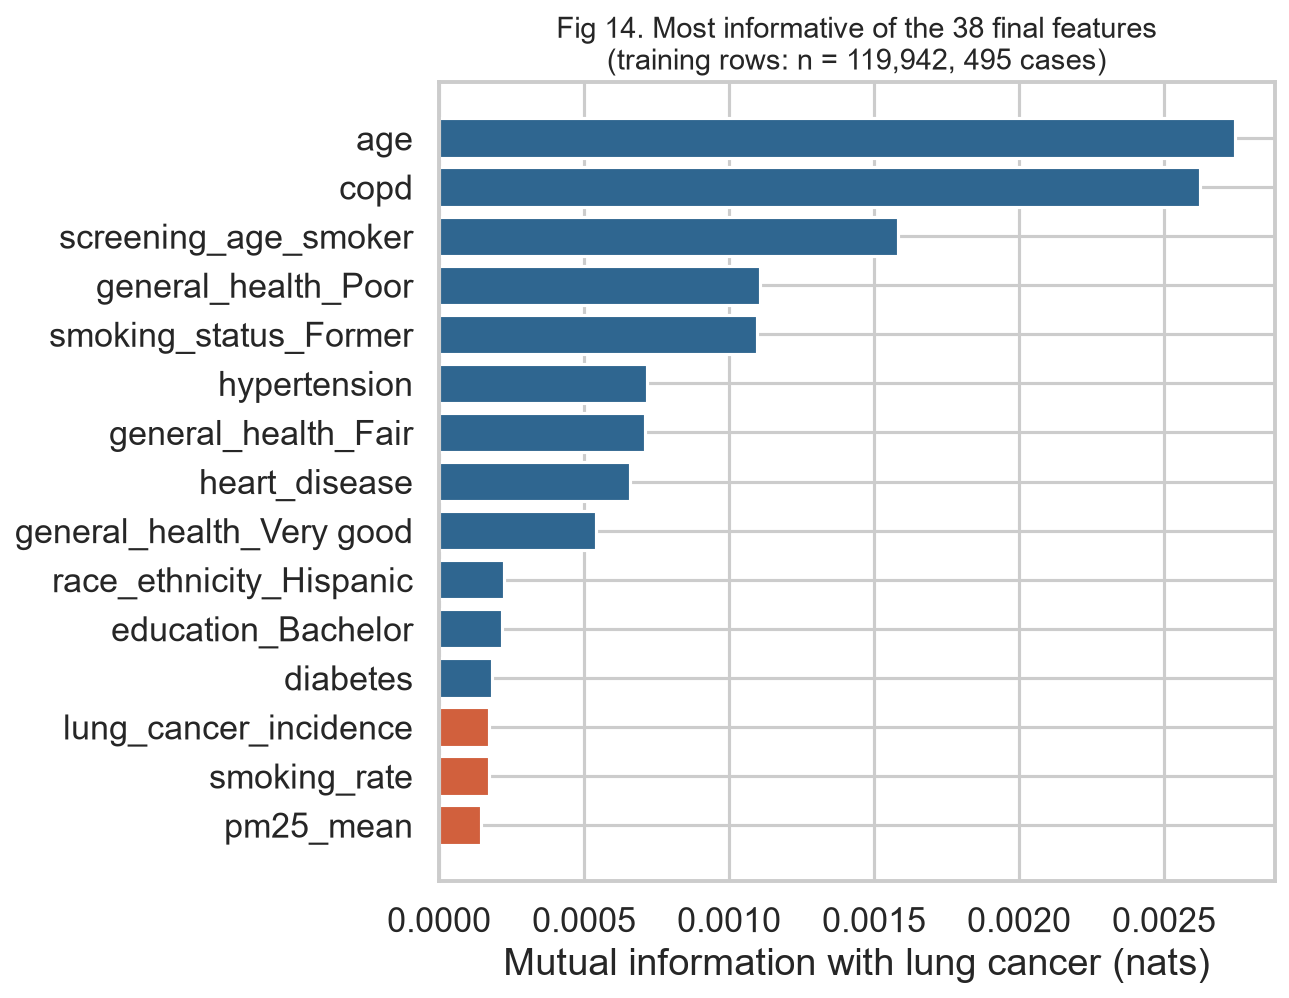
\includegraphics[width=0.65\textwidth]{fig14_feature_relevance}
\caption{Mutual information between each of the \nFeatures final features and the target on the training rows (top 15; $n$ = \nTrain adults, \nTrainCases cases). The three regional columns (orange) take the last three places; their nearly equal values reflect one shared region-year signal (\S\ref{sec:mi}).}\label{fig:mi}
\end{figure}

\subsection{Feature extraction with PCA}\label{sec:pca}

Feature selection keeps a subset of the original columns; feature extraction builds new ones. We tested whether Principal Component Analysis could compress the \nFeatures selected features without losing much information (Fig.~\ref{fig:scree}). Because the features have different units, we standardised all of them first -- equivalent to running PCA on the correlation matrix, as the course recommends~\cite{jolliffe,louati} -- and fitted both the scaler and the PCA on training rows only. Loadings are correlations between a feature and a component; only loadings with an absolute value of at least 0.40, the threshold used in the course, are listed in Table~\ref{tab:pca}.

\begin{figure}[htbp]
\centering
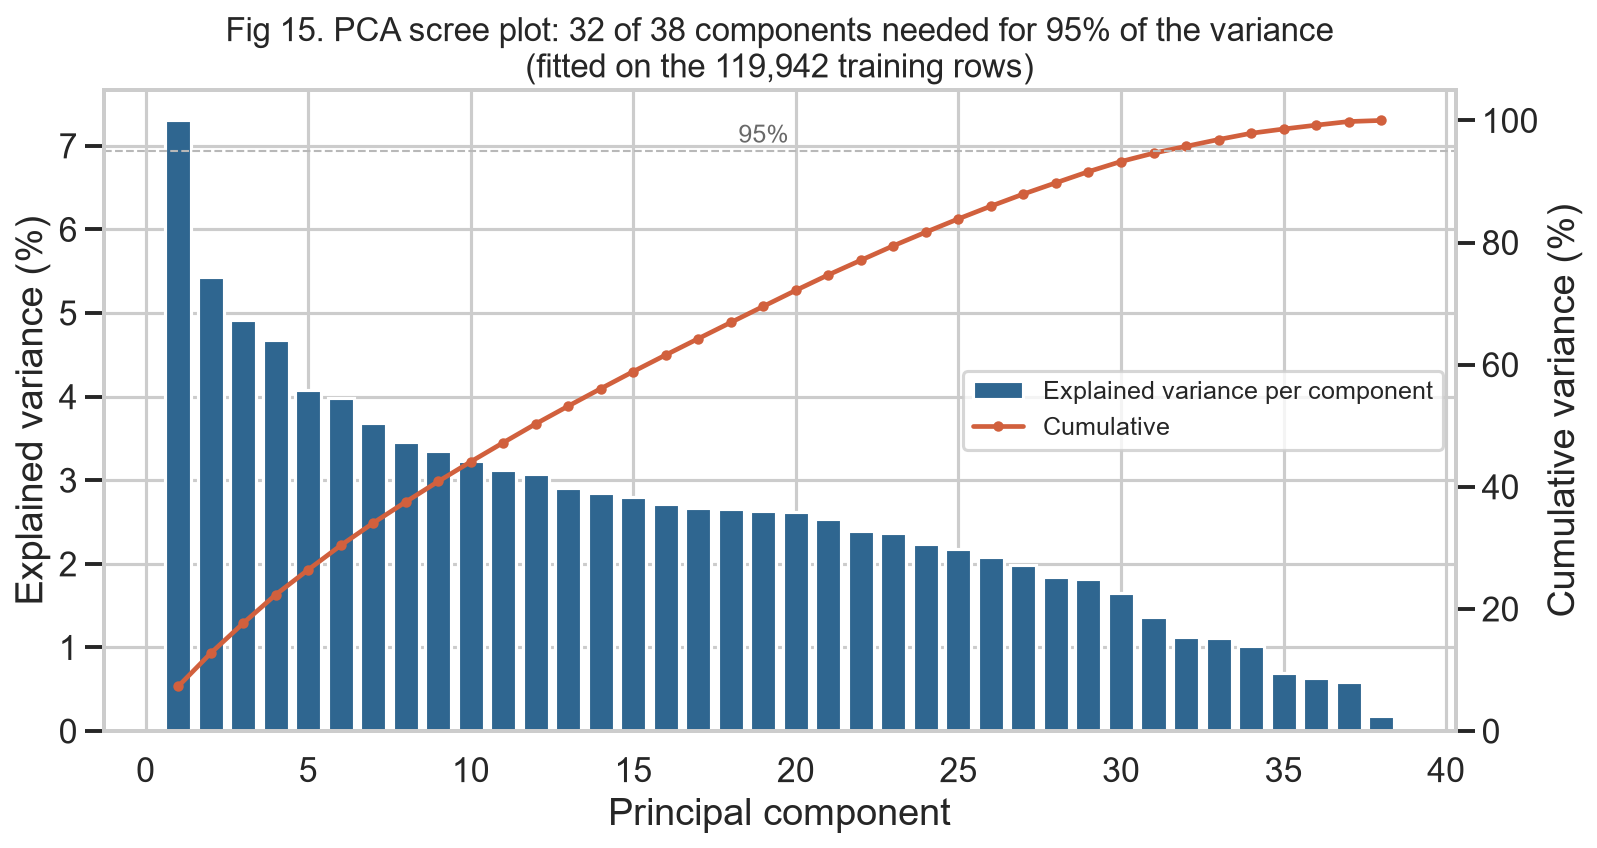
\includegraphics[width=0.8\textwidth]{fig15_pca_scree}
\caption{PCA scree plot (fitted on the \nTrain training rows): explained variance per component (bars) and cumulative variance (line). \pcaNinetyFive of \nFeatures components are needed to keep 95\% of the variance.}\label{fig:scree}
\end{figure}

\begin{table}[htbp]
\centering\small
\caption{PCA summary (fitted on the \nTrain training rows).}\label{tab:pca}
\begin{tabularx}{\textwidth}{>{\raggedright\arraybackslash}p{5.2cm} >{\raggedright\arraybackslash}X}
\toprule
Quantity & Value \\
\midrule
Variance explained by PC1 / PC2 / PC3 & 7.3\% / 5.4\% / 4.9\% (2.6\% expected per component if all features were unrelated) \\
Components needed for 80\% / 90\% / 95\% of the variance & 24 / 29 / 32 of 38 \\
Kaiser rule (eigenvalue $>$ 1) & 19 components \\
Components with almost zero variance (eigenvalue $<$ 0.01) & 0 (there were 8 with the previous 48 features: the dependencies removed by rule 4, \S\ref{sec:selection}) \\
Variance of the test rows kept by the first 32 components & 95.8\% (the PCA generalises; it never saw the test rows) \\
PC1 -- ``age and chronic-disease burden'' & hypertension +0.59, screening\_age\_smoker +0.57, age +0.57, diabetes +0.46, copd +0.45, heart\_disease +0.42 \\
PC2 -- ``skipped the smoking questions'' & screening\_age\_smoker\_unknown +0.86, ever\_ecigarette\_unknown +0.86 \\
PC3 -- ``older age vs current smoking and regional smoking level'' (mixed) & age +0.50, smoking\_rate $-$0.42 (next below 0.40: smoking\_status\_Current $-$0.39, ever\_ecigarette $-$0.38, lung\_cancer\_incidence $-$0.36, pm25\_mean $-$0.35) \\
\bottomrule
\end{tabularx}

\end{table}

\begin{figure}[htbp]
\centering
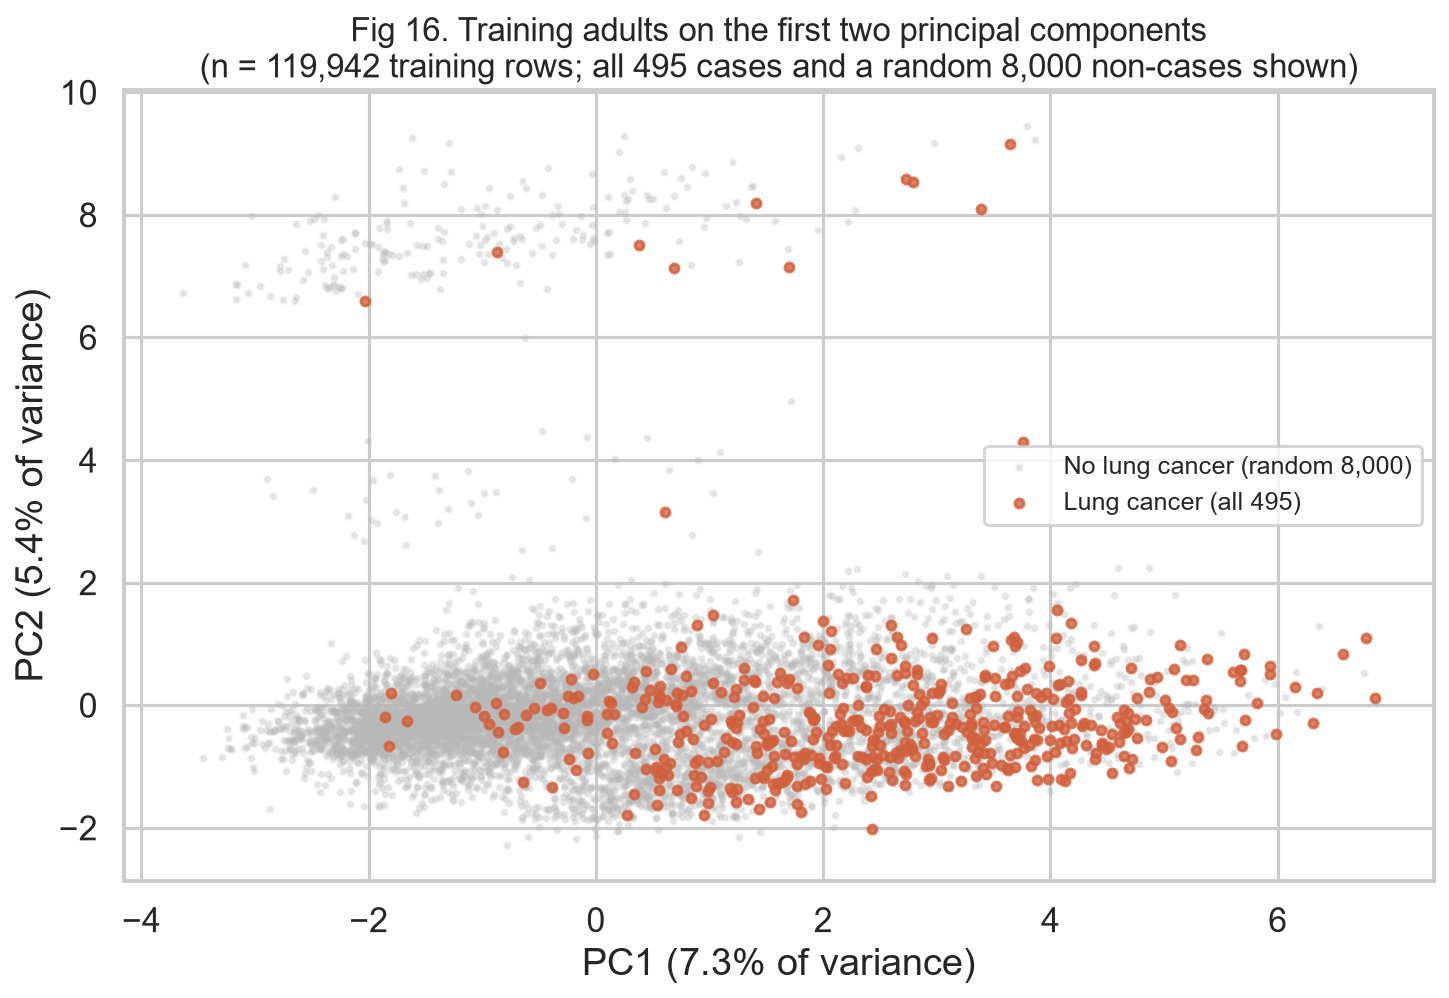
\includegraphics[width=0.75\textwidth]{fig16_pca_projection}
\caption{Training adults ($n$ = \nTrain) projected on the first two principal components: all \nTrainCases training cases (orange) and a random 8,000 non-cases (grey). The separate cloud at the top (high PC2) is the $\sim$2.8\% of adults who skipped the smoking questions.}\label{fig:projection}
\end{figure}

Lung-cancer cases sit on the high side of PC1 (Fig.~\ref{fig:projection}; mean score \pcaCaseMean vs $-0.01$ for other adults), which is the age-and-disease axis, but the two groups overlap heavily: two components cannot separate a rare outcome.

\textbf{Decision: we keep the original features.} Keeping 95\% of the variance would still need \pcaNinetyFive components -- only \pcaReduction\% fewer columns -- because the information is spread over many dimensions with no dominant one, which agrees with the weak correlations of Fig.~\ref{fig:featcorr} and the low VIFs of Table~\ref{tab:vif}. Interpretability also matters for a health question: an odds ratio for ``COPD'' means something to a clinician, a weight on ``PC4'' does not. Finally, most of our columns are 0/1 indicators, for which PCA, built for continuous data, is less natural (a method for mixed data, such as factor analysis of mixed data, would be the better tool if extraction were needed). The PCA is kept as an option to compare in the modelling phase, especially for distance-based methods such as $k$-nearest neighbours or clustering, which suffer most from many dimensions. The previous version of the feature set had eight near-zero directions. They are gone because rule 4 removed the dependencies behind them (the comorbidity count, one reference category per one-hot group, the region dummies), and that is also why the count of components dropped: an exact dependency is a zero-variance direction that carries no information.

\subsection{The final feature set and how it serves the objectives}\label{sec:final}

The \nFeatures final features are listed by group, with the reference category of every one-hot group, in Table~\ref{tab:comp-groups} (Section~\ref{sec:data}; full list in Appendix~\ref{app:features}).

\begin{itemize}
  \item It carries what the EDA found to matter -- age, smoking, COPD and the other chronic conditions (whose sum, \file{comorbidity_count}, stays in the clean dataset for the EDA only) -- in model-ready form, with no missing values and no exact or near-exact multicollinearity (maximum VIF \maxVIFshort).
  \item It links the dataset to the real clinical rule through \file{screening_age_smoker}, the baseline any future model must beat (Table~\ref{tab:screening}).
  \item It is leakage-free by construction and by check: every learned step saw training rows only, so the test score of a future model will be an honest estimate.
  \item It keeps the regional context for an ablation test rather than discarding it on the basis of four regions.
\end{itemize}

\textbf{Features we are cautious about.} \file{general_health}, BMI, current smoking status and the ``ever told'' conditions may partly be consequences of a cancer diagnosis (\S\ref{sec:sociodemo}). A model leaning on them would mostly recognise people who are already sick rather than give an early risk indication. We keep them, but plan to compare models with and without them. Race/ethnicity is kept to describe the population and to allow a fairness audit of any future model, not because race is a cause of lung cancer.

\textbf{Reading the dummies.} Every dummy is read against its group's reference category (Table~\ref{tab:comp-groups}). For smoking, the reference group \emph{Never} also contains the 2.6\% of adults whose smoking status is unknown. Their own dummy was dropped as a near-duplicate of \file{screening_age_smoker_unknown} ($r = 0.96$, rule 3), so that flag is the \textbf{only} feature that tells a model these adults are not known never-smokers. It must stay in any model that uses the smoking dummies, and an adjusted odds ratio for \emph{Current} or \emph{Former} smoking should be described as ``vs never or unknown, holding the unknown flag fixed''.
